\documentclass[11pt]{article}
\usepackage[margin=1in]{geometry} 
\usepackage{amsmath,amsthm,amssymb,amsfonts}

\usepackage{mathpazo}
\usepackage{euler}
\usepackage{xcolor}
\usepackage{tikz}
\usetikzlibrary{matrix}

\newcommand{\N}{\mathbb{N}}
\newcommand{\Z}{\mathbb{Z}}
\newcommand{\Q}{\mathbb{Q}}
\newcommand{\R}{\mathbb{R}}
\newcommand{\C}{\mathbb{C}}
\newcommand{\im}{\operatorname{im}}
\newcommand{\eps}{\varepsilon}

\newcommand{\paint}[2]{\color{#1}{#2}}
\definecolor{purple}{RGB}{129, 0, 125}

\renewcommand*{\proofname}{\paint{purple}{Demostraci\'on}}
\newenvironment{theorem}[2][Teorema]{\begin{trivlist}
\item[\hskip \labelsep {\bfseries #1}\hskip \labelsep {\bfseries #2.}]}{\end{trivlist}}
\newenvironment{lemma}[2][Lema]{\begin{trivlist}
\item[\hskip \labelsep {\bfseries #1}\hskip \labelsep {\bfseries #2.}]}{\end{trivlist}}
\newenvironment{exercise}[2][Ejercicio]{\begin{trivlist}
\item[\hskip \labelsep \paint{purple}{{\bfseries #1}}\hskip \labelsep {\bfseries #2.}]}{\end{trivlist}}
\newenvironment{reflection}[2][Resoluci\']{\begin{trivlist}
\item[\hskip \labelsep {\bfseries #1}\hskip \labelsep {\bfseries #2.}]}{\end{trivlist}}
\newenvironment{proposition}[2][Proposici\'on]{\begin{trivlist}
\item[\hskip \labelsep {\bfseries #1}\hskip \labelsep {\bfseries #2.}]}{\end{trivlist}}
\newenvironment{corollary}[2][Corolario]{\begin{trivlist}
\item[\hskip \labelsep {\bfseries #1}\hskip \labelsep {\bfseries #2.}]}{\end{trivlist}}

%-----------------------

\title{\paint{purple}{Geometr\'ia Diferencial}}
\author{\paint{purple}{Guido Arnone}}
\date{}

\begin{document}

\maketitle

\begin{exercise}{5} Muestre que los siguientes espacios son variedades diferenciales y determine sus
dimensiones. 
\begin{itemize}
\item[(i)] $\mathsf{SL}(n,\C)$ el conjunto de las matrices complejas de tama\~{n}o $n \times n$ y determinante $1$.
\end{itemize}
\end{exercise}
\begin{proof} Hacemos cada caso por separado.
\begin{itemize} 
\item[(i)] Afirmamos primero que la funci\'on $\det : \mathsf{M}_n\C \to \C$ es diferenciable. Eso es porque dada una matriz compleja $A = (X_{ij}+iY_{ij})_{ij}$, luego $\det A$ es un polinomio con coeficientes en $\C$ en funci\'on de cada $X_{ij}, Y_{ij}$,
\begin{align}
\det((X_{ij}+iY_{ij})_{i,j}) = \sum_{\sigma \in \mathbb{S}_n}sgn(\sigma)(X_{1\sigma(1)}+iY_{1\sigma(1)}) \cdots (X_{n \sigma(n)}+iY_{n\sigma(n)}).
\end{align}
Tomando partes reales e imaginarias tenemos que $\det A = \Re(\det A) + i \Im(\det A)$ con $\Re(\det), \Im(\det)$ dos polinomios ahora de valores reales. Identificando $\mathsf{M}_n\C \equiv \R^{2n^2}$ y $C \equiv R^2$ via homeomorfismos $\Phi : (X_{ij}+iY_{ij})_{i,j} \mapsto (X_1, \dots, X_{n^2}, Y_1, \dots, Y_{n^2})$ y $\phi : z \mapsto (\Re(z), \Im(z))$ luego $\paint{purple}{(2)}$ nos dice que en el siguiente diagrama,
\begin{center}
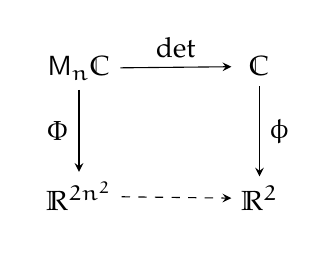
\begin{tikzpicture}
  \matrix (m) [matrix of math nodes,row sep=3em,column sep=4em,minimum width=2em]
  {
     \mathsf{M}_n\C & \C \\
     \R^{2n^2} & \R^2 \\};
  \path[-stealth]
    (m-1-1) edge node [above] {$\det$} (m-1-2)
            edge node [left] {$\Phi$} (m-2-1)
    (m-1-2) edge node [right] {$\phi$} (m-2-2)
    (m-2-1) edge [dashed] node [below] {} (m-2-2);
\end{tikzpicture}
\end{center}
la flecha punteada es diferenciable pues es un polinomio para cada coordenada de $\R^2$. A su vez, $\{(\mathsf{M}_n\C,\Phi)\}$ y $\{(\C,\phi)\}$ son  atlas, lo que prueba que $\det$ es diferenciable. Ahora bien, por definici\'on es $\mathsf{SL}(c,\C) = \det^{-1}(\{1\})$ y podemos apelar luego al teorema de valores regulares, viendo que el diferencial de $\det$ sea sobreyectivo en cada matriz $A \in \mathsf{SL}(n,\C)$.
\end{itemize}
\end{proof}
\begin{exercise}{7} Sean $M$ y $N$ variedades de dimensiones $m$ y $n$, respectivamente. Probar que:
\begin{itemize}
\item[(a)] El espacio producto $M \times N$ tiene una estructura natural de
variedad diferenciable de dimensi\'on $m+n$ y con respecto a esta estructura
las proyecciones $p_1:M\times N\to M$ y $p_2:M\times N\to N$ son funciones diferenciables.
\item[(b)] Si $P$ es una variedad y $f:P\to M$ y $g:P\to N$ son funciones
diferenciables, entonces existe exactamente una funci\'on diferenciable $h:P\to M\times N$ tal que $p_1\circ h=f$ y $p_2\circ h=g$.
\end{itemize}
\end{exercise}
\begin{proof} Hacemos cada inciso por separado:
\begin{itemize}
\item [(a)] Dotamos a $M \times N$ de la topolog\'ia producto. Luego, $M \times N$ es Hausdorff ya que es producto de espacios Hausdorff. Como $M$ y $N$ son variedades, tienen bases numerables $\mathcal{B}_M, \mathcal{B}_N$ respectivamente y entonces el conjunto numerable $\tilde{\mathcal{B}} = \{U \times V : U \in \mathcal{B}_M, V \in \mathcal{B}_N\}$ es base de $M \times N$. En efecto, si $A \subseteq M \times N$ es abierto y $(x,y) \in A$, existe luego un abierto b\'asico $(x,y) \in U \times V \subset A$. Como $\mathcal{B}_N$ y $\mathcal{B}_M$ son bases, tenemos abiertos $x \in U_0 \subseteq U \in \mathcal{B}_M$, $y \in V_0 \subseteq V \in \mathcal{B}_N$. Por lo tanto, $(x,y) \in U_0 \times V_0 \subseteq U \times V \subseteq A$, lo que prueba que $\tilde{\mathcal{B}}$ es base. Ahora veamos que $M \times N$ tiene una estructura diferenciable. Sean $\mathcal{A}_1 = \{(U_i,\varphi_i)\}_{i \in I}$ y $\mathcal{A}_2 = \{(V_j,\psi_j)\}_{j \in J}$ los atlas de $M$ y $N$ respectivamente. Para cada $(i,j) \in I \times J$, notamos $\varphi_i \times \psi_j$ a $(u,v) \in U_i \times V_j \mapsto (\varphi_i(u), \psi_j(v)) \in \varphi_i(U_i) \times \psi(V_j)$ y definimos luego
\begin{align*}
\mathcal{A} := \{(U_i \times V_j,\varphi_i \times \psi_j) \}_{(i,j) \in I \times J}.
\end{align*}
Veamos que este es un atlas para $M \times N$. Como la topolog\'ia en $M \times N$ es la producto cada $U_i \times V_j$ es abierto, y por otro lado, las funciones $\varphi_i \times \psi_j$ son homeomorfismos al ser producto de homeomorfismos. Adem\'as, dado que los abiertos $(U_i)_{i \in I}$ y $(V_j)_{j \in J}$ cubren $M$ y $N$ respectivamente, es
\begin{align*}
\bigcup_{(i,j) \in I \times J} U_i \times V_j = \bigcup_{i \in I} U_i \times \bigcup_{j \in J} V_j = M \times N.
\end{align*}
Finalmente, si $\varphi_i \times \psi_j$  y $\varphi_k \times \psi_l$ son cartas de $\mathcal{A}$, notando
\begin{align*}
W := (U_i \times V_j) \cap (U_k \times V_l) = (U_i \cap U_k) \times (V_j \times V_l)
\end{align*}
tenemos que la composici\'on 
\begin{align}
(\varphi_i \times \psi_j)|_W \circ ((\varphi_k \times \psi_l)|_W)^{-1} : (\varphi_k \times \psi_l)(W) \mapsto (\varphi_i \times \psi_j)(W)
\end{align}
verifica
\begin{align*}
(\varphi_i \times \psi_j)|_W \circ ((\varphi_k \times \psi_l)|_W)^{-1}(x,y) & = (\varphi_i \times \psi_j) \circ (\varphi^{-1}_k \times \psi^{-1}_l) (x,y)\\
& =(\varphi_i\varphi^{-1}_k(x), \psi_j\psi^{-1}_l(y))
\end{align*}
para cada $(x,y) \in (\varphi_k \times \psi_l)(W) = \varphi_k(U_i \cap U_k) \times \psi_l(V_j \times V_l)$. Como por hip\'otesis tanto $\varphi_i\varphi^{-1}_k$ como $\psi_j\psi^{-1}_l$ son funciones diferenciables entre abiertos eucl\'ideos, es entonces $\varphi_i\varphi^{-1}_k \times \psi_j\psi^{-1}_l$ diferenciable y a la vez coincide con $\paint{purple}{(2)}$, lo que termina de probar que $\mathcal{A}$ dota a $M \times N$ de una estructura diferenciable. Los abiertos $U_i \times V_j$ son en particular abiertos de $\mathbb{R}^{n+m}$ lo que dice que $\dim M \times N = \dim M + \dim N = m+n$. Ahora veamos que las proyecciones son diferenciables. Fijamos $(x,y) \in M \times N$ y sea $(U_i \times V_j, \varphi_i  \times \psi_j)$ una carta en con $x \in U_i, y \in V_j$. Luego por construcci\'on de $\mathcal{A}$ sabemos que $\varphi_i$ es carta de $M$ con $x = p_1(x,y) \in p_1(U_i \times V_j) = U_i$ y $\psi_j$ es carta de $N$ con $y = p_2(x,y) \in p_2(U_i \times V_j) = V_j$. Basta entonces con probar que $\varphi_i p_1 (\varphi_i \times \psi_j)^{-1}$ y $\psi_j p_2 (\varphi_i \times \psi_j)^{-1}$ son diferenciables. \'Esta \'ultima es exactamente la proyecci\'on en la segunda coordenada $\tilde{p}_2 : \varphi_i(U_i) \times \psi_j(V_j) \to \psi_j(V_j)$, ya que si $(x,y) \in \varphi_i(U_i) \times \psi_j(V_j)$ entonces $\psi_j p_2 (\varphi_i \times \psi_j)^{-1}(x,y) = \varphi_i p_2 (\varphi_i^{-1}(x),\psi^{-1}_j(y)) = \psi_j(\psi^{-1}_j(y)) = y$. Similarmente $\varphi_i p_1 (\varphi_i \times \psi_j)^{-1}$ es la proyecci\'on de $\varphi_i(U_i) \times \psi_j(V_j)$ en la primera coordenada, y as\'i vemos que ambas proyecciones son diferenciables.
\item[(b)] Veamos en primer lugar que existe una tal funci\'on. Consideramos 
\begin{align*}
h : p \in P \mapsto (f(p),g(p)) \in M \times N
\end{align*}
que verifica $p_1h(p) = p_1(f(p), g(p)) = f(p)$ y $p_2h(p) = g(p)$. Sea $\mathcal{A}' = \{(\mu_k,W_k)\}_{k \in K}$ un atlas maximal de $P$ y fijemos $p \in P$. Tomamos a continuaci\'on $W_k \ni p$ y $U_i \times V_j \ni h(p) = (f(p),g(p))$ abiertos de $P$ y $M \times N$ respectivamente, correspondientes a cartas $(\mu_k,W_k)$ y $(\varphi_i \times \psi_j, U_i \times V_j)$. Ahora, veamos que $(\varphi_i \times \psi_j)h \mu_k^{-1}$ es diferenciable. Como punto a punto tenemos que
\begin{align*}
(\varphi_i \times \psi_j)h \mu_k^{-1}(z) = (\varphi_i \times \psi_j)(f(\mu_k^{-1}(z)) , g(\mu_k^{-1}(z))) = (\varphi_i f(\mu_k^{-1}(z)),\psi_j g(\mu_k^{-1}(z)))
\end{align*}
para cada $z \in \mu_k(W_k)$ y tanto $\varphi_if\mu_k^{-1}$ como $\psi_jg\mu_k^{-1}$ son diferenciables pues $f$ y $g$ son diferencables, consecuentemente $(\varphi_i \times \psi_j)h \mu_k^{-1}$ es diferenciable. Con respecto a la unicidad, est\'a dada a un nivel de conjuntos: si $\tilde{h} : P \to M \times N$ cumple $p_1\tilde{h} = f$ y $p_2\tilde{h} = g$, luego notando $\tilde{h}(p) = (\tilde{h}_1(p), \tilde{h}(p)_2)$ tenemos que 
\begin{align*}
f(p) = p_1\tilde{h} = \tilde{h}_1(p)
\end{align*}
y
\begin{align*}
g(p) = p_2\tilde{h} = \tilde{h}_2(p)
\end{align*}
as\'i que $\tilde{h}(p) = (f(p),g(p)) = h(p)$, para todo $p \in P$.
\begin{center}
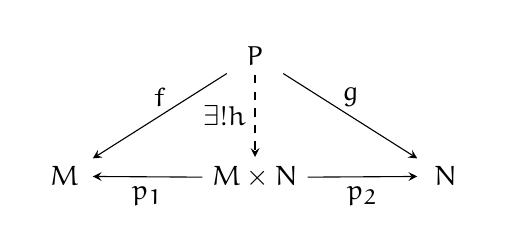
\begin{tikzpicture}
  \matrix (m) [matrix of math nodes,row sep=3em,column sep=4em,minimum width=2em]
  {
     & P &  \\
     M & M \times N & N \\};
  \path[-stealth]
    (m-1-2) edge node [above] {$f$} (m-2-1)
            edge [dashed] node [left] {$\exists ! h$} (m-2-2)
            edge node [above] {$g$} (m-2-3)
    (m-2-2) edge node [below] {$p_1$} (m-2-1)
    (m-2-2) edge node [below] {$p_2$} (m-2-3);
\end{tikzpicture}
\end{center}
\end{itemize}
\end{proof}
\end{document}
